\section{Sviluppi successivi}

Al fine di ottenere migliori risultati nella fase di classificazione, sono state apportate alcune modifiche all'elaborato e considerato un modo migliore di trattare il dataset a disposizione.

\subsection{Analisi}

L'analisi effettuata in precedenza evidenziava che, trattando le immagini nella loro interezza (seppure con la possibilità di una variazione di scala), alcuni dei \emph{pattern} fossero difficilmente classificabili.
Questo può dipendere principalmente da diversi fattori, primo fra tutti la grande varietà di cellule presenti all'interno di uno stesso vetrino: subbene infatti fossero etichettati come un'unica entità, non tutte le cellule presenti si mostravano allo stesso modo, evidenziando in alcuni punti pattern ben diversi da quello di riferimento (vedi Figura \ref{fig:errors}). Questo fatto porta a \emph{confondere} il classificatore che vedrà come pattern possibili più di un unico risultato.

\begin{figure}[H] 
  \centering
    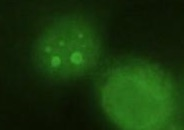
\includegraphics[width=0.4\textwidth]{images/errori.jpg}
    \caption{{\small \textit{Cellule con diverso pattern nella stessa immagine}}}
   \label{fig:errors}
\end{figure}

In aggiunta al problema sopraelencato i risultati evidenziano una particolare difficoltà nella classificazione di alcuni pattern: \emph{nucleolare}, \emph{granulare} e \emph{citoplasmico} (Tabella \ref{table:1}). Questo può dipendere dalla loro effettiva somiglianza visiva, dalla bassa risoluzione con cui vengono trattate le immagini (in caso di scala) oppure da un non adatto modello di features usato per la loro descrizione.

\subsection{Miglioramento del dataset}

Date le problematiche evidenziate, una possibile soluzione era quella di utilizzare un dataset in cui ciascuna cellula, e non più l'intero vetrino, fosse etichettata singolarmente. 
In questo caso, nella fase di estrazione delle features, è possibile mantenendo accettabile il tempo di computazione necessario, provvedere a ingrandire le immagini così da consentire una miglior distinzione tra pattern singoli.

Il dataset è dunque ora composto da un totale di 1455 immagini di cellule singolarmente etichettate in 6 diversi pattern:
\begin{itemize}
\item Omogeneo
\item Punteggiato
\item Finemente punteggiato
\item Centromero
\item Nucleolare
\item Citoplasmico
\end{itemize}

Come si nota, a differenza del precedente esperimento, in questo caso il pattern \emph{punteggiato} è stato diviso nelle due sue forme più comuni ed è stato eliminato il pattern \emph{negativo}, non rilevante ai fini della classificazione in quanto completamente (o quasi) nero.

\subsubsection{Risultati}

I risultati ottenuti con queste modifiche sono molto migliori dei precedenti, andando a migliorare di quasi dieci punti percentuali l'accuratezza ottenuta in precedenza.

I risultati sono ottenuti cross-validando il dataset in 10 sottoparti. La classificazione è fatta tramite SVM, utilizzando però la libreria open-source \emph{libSVM}\footnote{LibSVM, \emph{A Library for Support Vector Machines}, https://www.csie.ntu.edu.tw/~cjlin/libsvm/} alla versione 3.2. L'utilizzo di questa libreria ha consentito di poter meglio personalizzare i parametri del classificatore e presenta una migliorazione nei tempi di computazione rispetto alla versione implementata nativamente in Matlab.

I risultati ottenuti vengono presentati nella matrice di confusione e nella tabella

\begin{figure}[H] 
  \centering
    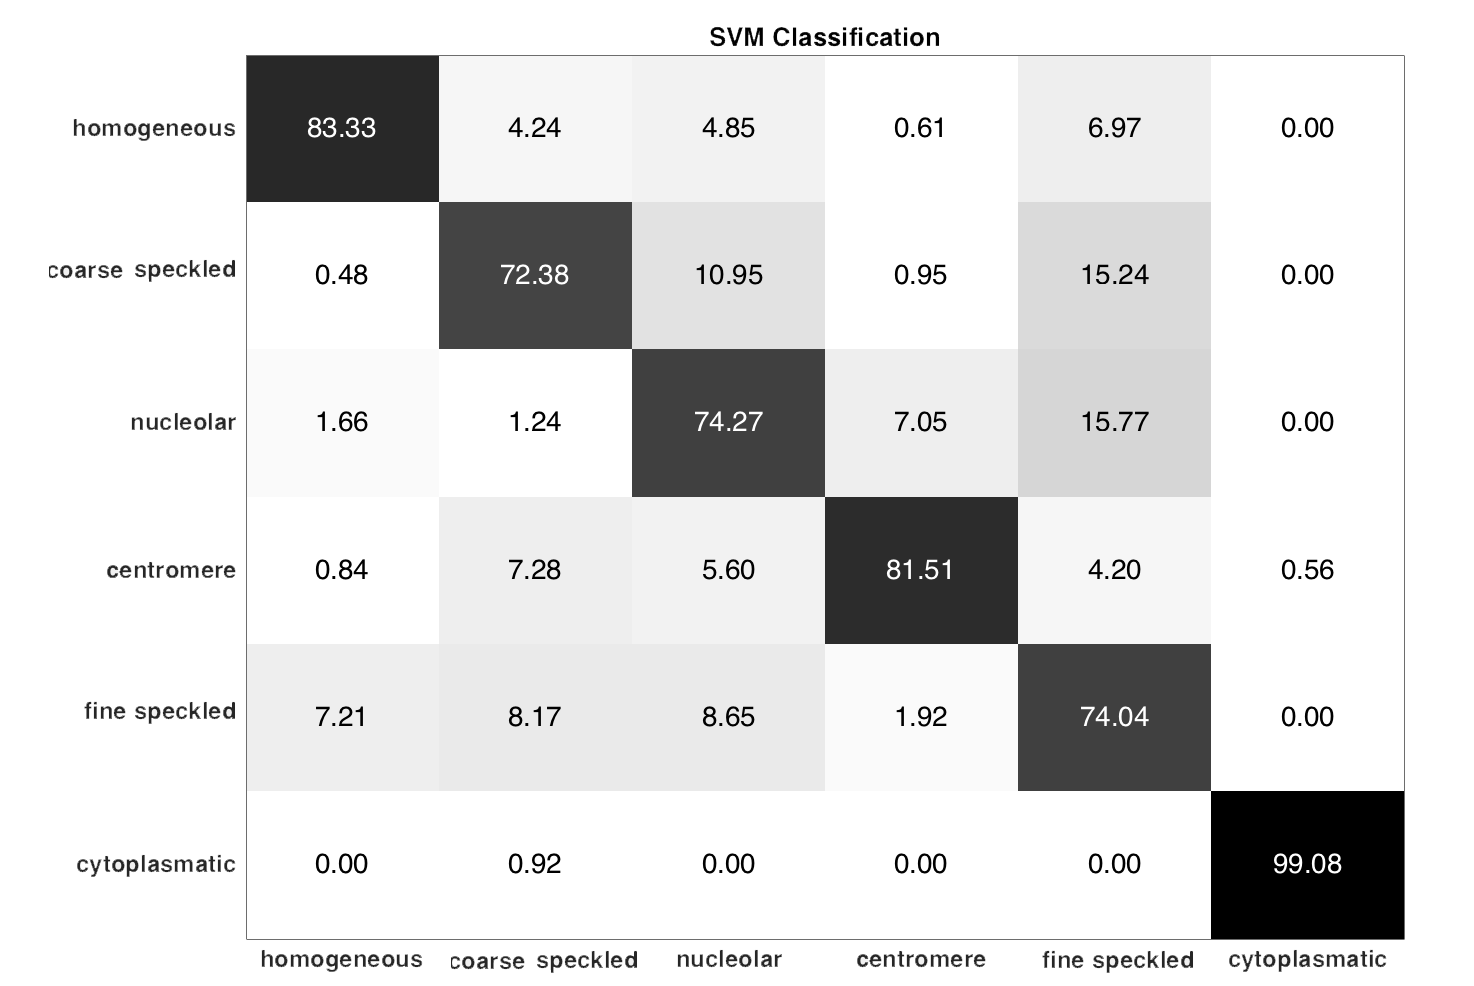
\includegraphics[width=0.9\textwidth]{images/conf_mat_2.png}
    \caption{{\small \textit{Matrice di confusione}}}
\end{figure}



